\documentclass[border=10pt]{standalone}
\usepackage{tikz}
\usetikzlibrary{arrows.meta, shapes, calc}

\begin{document}
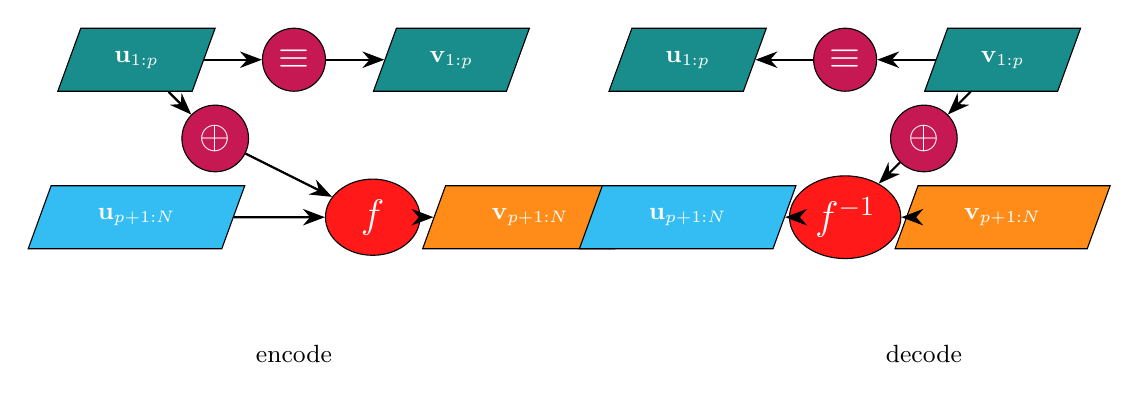
\begin{tikzpicture}[
    node distance=1.5cm,
    block/.style={draw, fill=teal!90, text=white, minimum width=1.5cm, minimum height=0.8cm, trapezium, trapezium left angle=70, trapezium right angle=110, text centered, font=\bfseries\small},
    block_blue/.style={draw, fill=cyan!80, text=white, minimum width=1.5cm, minimum height=0.8cm, trapezium, trapezium left angle=70, trapezium right angle=110, text centered, font=\bfseries\small},
    block_orange/.style={draw, fill=orange!90, text=white, minimum width=1.5cm, minimum height=0.8cm, trapezium, trapezium left angle=70, trapezium right angle=110, text centered, font=\bfseries\small},
    op_circle/.style={draw, fill=purple!90, text=white, circle, minimum size=0.8cm, text centered, font=\Large},
    op_oval/.style={draw, fill=red!90, text=white, ellipse, minimum width=1.2cm, minimum height=0.8cm, text centered, font=\Large},
    arrow/.style={thick, -{Stealth[scale=1.2]}},
    label/.style={font=\small, anchor=north, yshift=-0.5cm}
]

% Encode Diagram (Left)
\node[block] (u1p) at (0, 0) {$\mathbf{u}_{1:p}$};
\node[block_blue] (up1N) at (0, -2) {$\mathbf{u}_{p+1:N}$};
\node[op_circle] (eq) at (2, 0) {$\equiv$};
\node[op_circle] (oplus) at (1, -1) {$\oplus$};
\node[op_oval] (f) at (3, -2) {$f$};
\node[block] (v1p) at (4, 0) {$\mathbf{v}_{1:p}$};
\node[block_orange] (vp1N) at (5, -2) {$\mathbf{v}_{p+1:N}$};

% Arrows for Encode
\draw[arrow] (u1p) -- (eq);
\draw[arrow] (u1p) -- (oplus);
\draw[arrow] (up1N) -- (f);
\draw[arrow] (oplus) -- (f);
\draw[arrow] (eq) -- (v1p);
\draw[arrow] (f) -- (vp1N);

% Label for Encode
\node[label] at (2, -3) {encode};

% Decode Diagram (Right)
\node[block] (u1p_dec) at (7, 0) {$\mathbf{u}_{1:p}$};
\node[block_blue] (up1N_dec) at (7, -2) {$\mathbf{u}_{p+1:N}$};
\node[op_circle] (eq_dec) at (9, 0) {$\equiv$};
\node[op_circle] (oplus_dec) at (10, -1) {$\oplus$};
\node[op_oval] (f_inv) at (9, -2) {$f^{-1}$};
\node[block] (v1p_dec) at (11, 0) {$\mathbf{v}_{1:p}$};
\node[block_orange] (vp1N_dec) at (11, -2) {$\mathbf{v}_{p+1:N}$};

% Arrows for Decode
\draw[arrow] (v1p_dec) -- (eq_dec);
\draw[arrow] (v1p_dec) -- (oplus_dec);
\draw[arrow] (vp1N_dec) -- (f_inv);
\draw[arrow] (oplus_dec) -- (f_inv);
\draw[arrow] (eq_dec) -- (u1p_dec);
\draw[arrow] (f_inv) -- (up1N_dec);

% Label for Decode
\node[label] at (10, -3) {decode};

\end{tikzpicture}
\end{document}
